\styledchapter[Architecturale ontwerp van de oplossing]{architecturale-ontwerp}
Nu het bekend is hoe ML pipelines en orkestratietools werken, kan er gekeken worden naar hoe de PoC architecturaal eruit gaat zien. De technische tekeningen laten zien hoe verschillende componenten in de PoC interacteert met elkaar en met componenten buiten de scope van de PoC. De tekeningen zijn gemaakt volgens het C4 model \cite{c4-model}. In dit hoofdstuk zal worden uitgelegd hoe C4 gelezen moet worden waarna de technische tekeningen wordt uitgelegd.

\section{Het C4 model}\label{sec:ch6-het-c4-model}
Het C4 model is een notatietechniek om de architectuur van een systeem te communiceren en is bedacht door Simon Brown \cite{c4-model}. Bij het tekenen van de modellen wordt er gedacht in vier niveaus: context, containers, components en code. In \autoref{fig:ch6-c4-overview-example} is een voorbeeld van een C4 model te zien. De context level is het eerste niveau waarbij wordt gekeken naar het systeem, gebruikers en contexten buiten de scope. Het systeem binnen de scope kan uitgebreid worden door middel van de volgende niveau, containers. Dit niveau laat op een hoog niveau zien waar het systeem uit bestaat. Elk container kan verder verduidelijkt worden met het component niveau. Hierbij worden containers verder opgebroken in components. Het laatste niveau is de code niveau en wordt doorgaans weergegeven via een klassendiagram. 

\begin{figure}[hbt!]
  \centering
  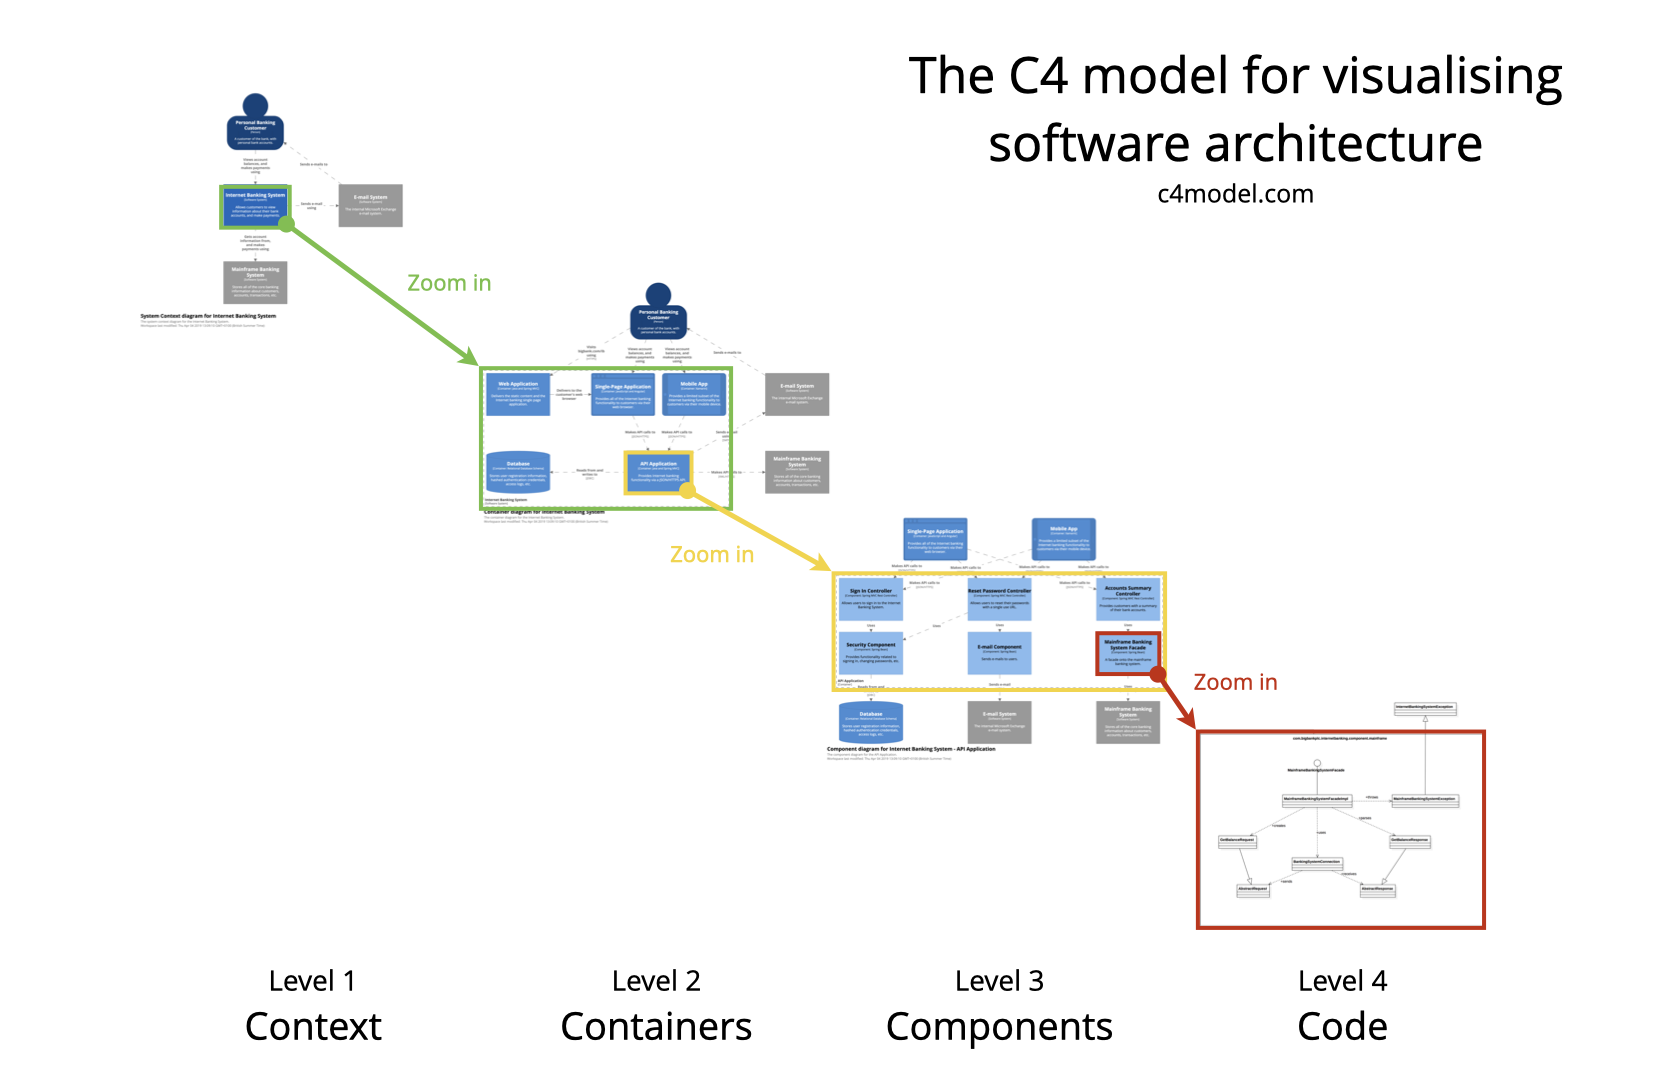
\includegraphics[width=0.99\textwidth]{chapter-6/c4-overview-example.png}
  \caption{Voorbeeld van een C4 model \cite{c4-model}.}
  \label{fig:ch6-c4-overview-example}
\end{figure}

\newpage

\section{Architecturaal ontwerp}\label{sec:ch6-architecturaal-ontwerp}
Op context niveau is het vrij simpel met het \acrfull{mlpa} systeem binnen de scope waarmee een developer interacteert en cloud computing platformen die buiten de scope vallen (\autoref{fig:ch6-c4-l1}). In deze diagram is ook te zien dat developers alleen gebruik maken van het systeem en indirect van cloud platformen. In de context diagram is ook een \acrfull{cli}/program te zien dat gebruik kan maken van de \acrshort{mlpa} systeem. Deze valt echter buiten de scope en is daarom aangegeven met een stippellijn.

\begin{figure}[hbt!]
  \centering
  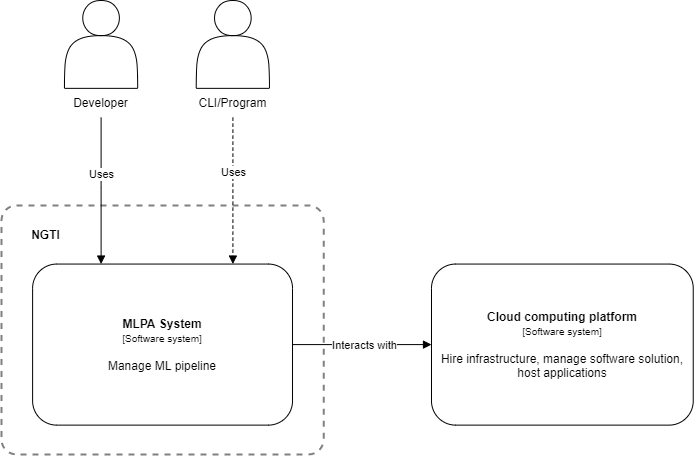
\includegraphics[width=0.65\textwidth]{chapter-6/C4-L1 - System Context diagram.png}
  \caption{Context niveau diagram van het architecturaal ontwerp.}
  \label{fig:ch6-c4-l1}
\end{figure}

In \autoref{fig:ch6-c4-l2} is de container niveau van het \Acrshort{mlpa} systeem te zien. Het systeem bestaat uit een \acrfull{spa} frontend, een Node.js met Express backend en een PostgreSQL database. Een developer krijgt van de backend de \Acrshort{spa} geserveerd waarmee waarmee een pipeline beheert kan worden. De frontend stuurt \Acrshort{api} requests naar de backend die vervolgens interacteert met de database en cloud platformen.

Voor de keuze van frameworks is rekening gehouden met de populariteit en kwaliteit van documentatie. Voor de populariteit is nogmaals de enquête van Stack Overflow geraadpleegd \cite{stack-overflow-survey-2020}. Volgens de resultaten scoren zowel React.js, Node.js en Express hoog \cite{stack-overflow-survey-2020-technology-web-frameworks} \cite{stack-overflow-survey-2020-popular-framework-libraries-tools}. Daarnaast hebben alle drie frameworks robuuste documentatie met references en tutorials \cite{reactjs-docs} \cite{nodejs-docs} \cite{expressjs-docs}.

\begin{figure}[hbt!]
  \centering
  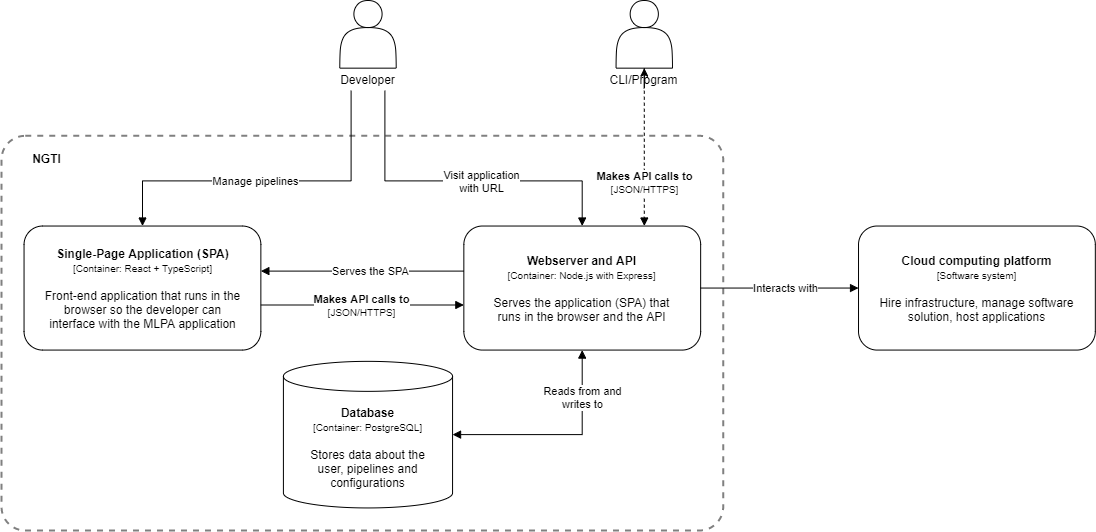
\includegraphics[width=0.99\textwidth]{chapter-6/C4-L2 - Container diagram.png}
  \caption{Container niveau diagram van het architecturaal ontwerp.}
  \label{fig:ch6-c4-l2}
\end{figure}

\newpage

Als laatste is de component overview van de \acrshort{spa} te zien in \autoref{fig:ch6-c4-l3-spa} en van de webserver met \acrshort{api} in \autoref{fig:ch6-c4-l3-nodejs}. De \acrshort{spa} bevat een \(AuthManager\) component dat controleert of de developer is ingelogd. Als dat het geval is, stuurt de \(Router\) component de developer door naar de \(Dashboard\), \(Pipeline overview\) of \(Pipeline details\) pagina.

\begin{figure}[hbt!]
  \centering
  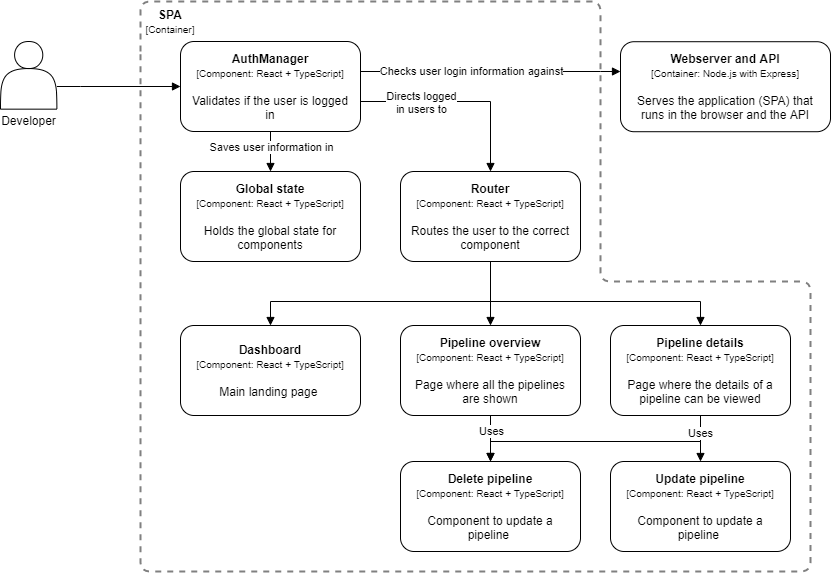
\includegraphics[width=0.8\textwidth]{chapter-6/C4-L3 - Component diagram - SPA.png}
  \caption{\Acrfull{spa} component niveau diagram van het architecturaal ontwerp.}
  \label{fig:ch6-c4-l3-spa}
\end{figure}

De component diagram van het \acrshort{mlpa} systeem bevat het complexe gedeelte (\autoref{fig:ch6-c4-l3-nodejs}). Hier komt een \acrshort{api} request binnen in een \(Express Route\). De route maakt vervolgens gebruik van Pulumi en het database om taken uit te voeren zoals het starten van een pipeline, het uploaden van een dataset of de status van een run bekijken.

\begin{figure}[hbt!]
  \centering
  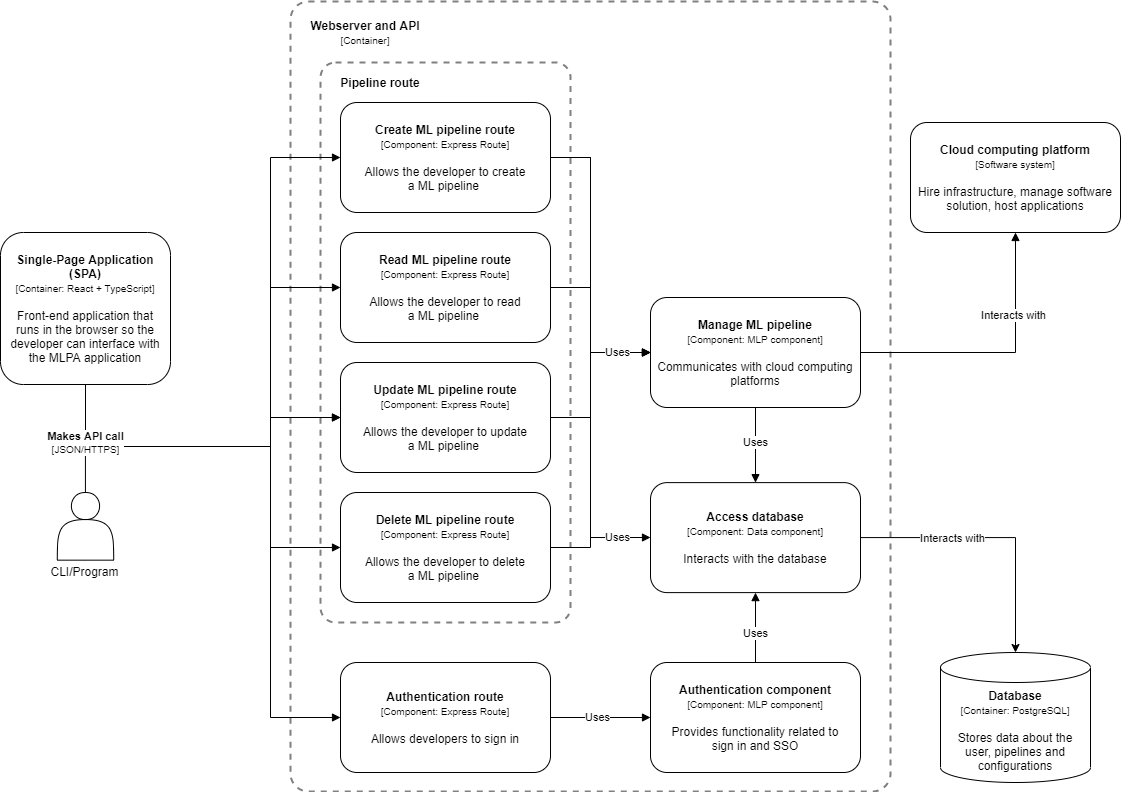
\includegraphics[width=0.99\textwidth]{chapter-6/C4-L3 - Component diagram - Webserver and API.png}
  \caption{Node.js server component niveau diagram van het architecturaal ontwerp.}
  \label{fig:ch6-c4-l3-nodejs}
\end{figure}

% De architectuur van de Node.js server is ontworpen met de separation of concerns principe in gedachte \cite{dijkstra-separation-of-concerns} \cite{solid-principle}. Dit betekent dat functies zoals het ophalen van pipeline-details opgebroken is kleinere functies. De functies bekommeren zich alleen om een functionaliteit. in [SUBKOP LINK] zal dit uitgelegd worden met voorbeelden.

De architectuur van de Node.js server is ontworpen volgens de repository-service pattern \cite{repository-service-pattern}. Dit is een pattern dat bepaalde zaken van elkaar scheid zodat het project onderhoudbaar blijft. In \autoref{sec:ch7-kwaliteit-van-de-code} zal dit uitgelegd worden met voorbeelden.

Diagrammen voor de laatste niveau, code, zijn achterwege gelaten door de vereiste tijd om de diagrammen te maken en het feit dat de diagrammen vaak tijdens het programmeerproces zullen veranderen. Brown geeft ook als advies om de diagrammen niet te maken of automatisch te laten genereren \cite{c4-model-faq}.

\newpage

\section{Sequence diagrammen}\label{sec:ch6-sequence-diagrammen}
Naast de C4 model diagrammen is het behulpzaam om uit te leggen wat er gebeurd als er een actie wordt uitgevoerd. Dit kan met behulp van sequence diagrammen. Voor belangrijke acties zoals het aanmaken of uitvoeren van een pipeline is een sequence diagram gemaakt. Daarnaast is een \acrfull{erd} gemaakt om de structuur van het database weer te geven. In deze kop wordt door een aantal diagrammen gelopen.

In \autoref{fig:ch6-c4-sd-create-pipeline} is te zien wat er gebeurt als een pipeline wordt aangemaakt. De developer stuurt een request naar de backend waar het wordt gevalideerd. De validatie sequence diagram is te vinden in bijlage \ref{appendix:validation-sequence-diagram}. De backend slaat vervolgens de gegevens op waarna, in parallel, een ingest server, model server en storage bucket worden aangemaakt. De ingest server zorgt voor de intake van datasets, de model traint het model en in de storage bucket wordt alle datasets en modellen opgeslagen. Als deze drie resources zijn aangemaakt, wordt de request voltooid.

\begin{figure}[hbt!]
  \centering
  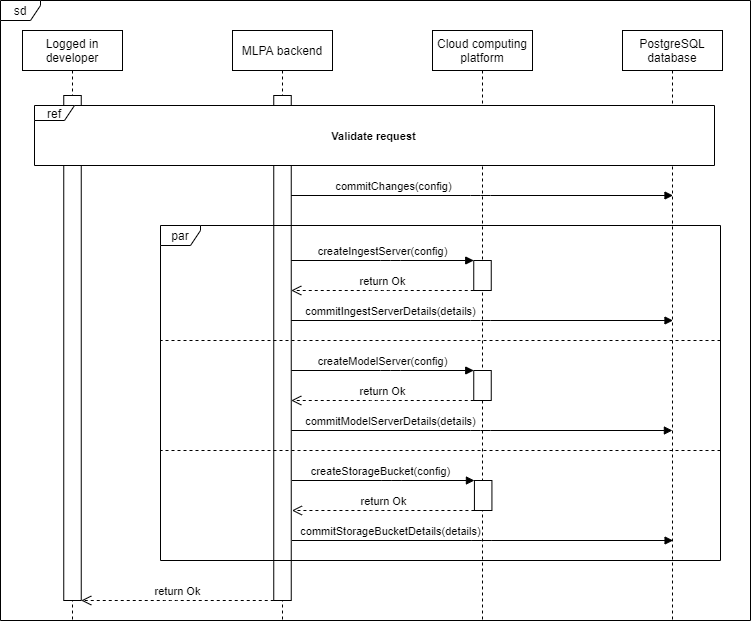
\includegraphics[width=0.99\textwidth]{chapter-6/C4-SD - Create pipeline.png}
  \caption{Sequence diagram van het aanmaken van een pipeline.}
  \label{fig:ch6-c4-sd-create-pipeline}
\end{figure}

\newpage

Een sequence diagram is gemaakt om te laten zien wat er gebeurt als een pipeline wordt gestart (\autoref{fig:ch6-c4-sd-start-pipeline}). De developer zal een request maken om de pipeline te starten. Om dit te doen stuurt de backend een request naar de cloud platform om een \acrfull{vm} te starten. Na het opstarten wordt het trainen van het model automatisch gestart. De backend past de status van de pipeline aan en voltooid de request. De developer weet nu dat een \acrshort{vm} is gestart en kan vragen voor de output van de \acrshort{vm}. In de output is te zien waar de \acrshort{vm} mee bezig is. Dit gebeurt continu totdat het model getraind is en de artefacten veilig zijn opgeslagen. Dit zijn afbeeldingen, modellen en datasets die bewaard moeten worden. Hierna zal de developer een laatste request sturen om de \acrshort{vm} te verwijderen en de status in het database aan te passen. 

\begin{figure}[hbt!]
  \centering
  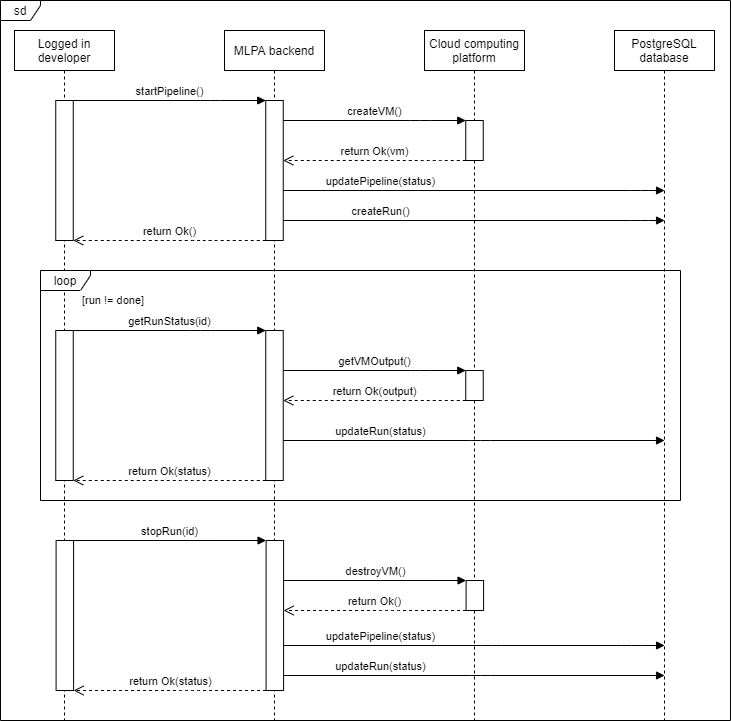
\includegraphics[width=0.99\textwidth]{chapter-6/C4-SD - Start pipeline.png}
  \caption{Sequence diagram van het starten van een pipeline.}
  \label{fig:ch6-c4-sd-start-pipeline}
\end{figure}

